\documentclass[fleqn,10pt]{physiome}
\usepackage{booktabs}
\usepackage{float}
\usepackage{tabularx}
\usepackage{placeins}
\usepackage{multirow}
\usepackage{lscape}
\usepackage{amsmath}
\usepackage{pdflscape}
\usepackage{rotating}
\articletype{Original}
\usepackage{xcolor,colortbl}
\newcolumntype{a}{>{\columncolor{gray}}c}
%% Choose from Original, Retrospective, Review, Letter
\title{Computational modeling of anoctamin 1 calcium-activated chloride channels
as pacemaker channels in interstitial cells of Cajal}

\author[1][l.noroozbabaee @auckland.ac.nz]{Leyla Noroozbabaee}
\author[1]{David P. Nickerson} 
\author[1a]{Peng Du}

\affil[1]{Auckland Bioengineering Institute, University of Auckland, New Zealand}
\affil[a]{Nominated from the primary publication authors to be a co-author.}

%% The following lines can be omitted when submitting;
%% information will be added by editors
\publicationdate{25 Dec 2022}
\editor{Karin Lundengård}
\curator{Weiwei Ai}
\submitteddate{10 Mars 2022}
\accepteddate{4 Dec 2022}
\citethisas{Noroozbabaee and Nickerson (2022)\\Computational modeling of anoctamin 1 calcium-activated chloride channels as pacemaker channels in interstitial cells of Cajal. Physiome.}{10.36903/physiome.21760691}

\begin{document}

\maketitle

\begin{abstract}
The system of equations and simulation results presented in \citet{lees2014computational} are verified and reproduced in the current paper. To demonstrate reproducibility, we here describe the model encoded in CellML and document the differences between our curated model and that published by \citeauthor{lees2014computational}.

\end{abstract}

\keywords{interstitial cells of Cajal, computational model, OpenCOR, CellML, ionic current}

\primarypubs[10.36903/physiome.21760691]{ref}{lees2014computational}

\section{Introduction}
\citet{lees2014computational} describes a biophysical computational model of anoctamin 1 (Ano 1) calcium-activated chloride channels (pacemaker channels in interstitial cells of Cajal). The current work involves the mathematical curation of the model in the CellML format \citep{doi:10.1177/0037549703040939}, which can reproduce the behaviour of each of the model's variations presented in \citet{lees2014computational}. Figure 2 in \citet{lees2014computational} is not included as it does not represent the introduced model's results. Additionally, some inconsistencies have been identified and are discussed in this work. A persistent workspace for this work is available in the Physiome Model Repository at \url{https://models.physiomeproject.org/workspace/83c}. The specific version of this implementation used to produce the presented results is included in the OMEX Archive \citep{bergmann_combine_2014}.

This implementation includes the Python source code to generate the model simulations in a `Simulations' directory. The corresponding CellML implementation is available in a `Experiments' directory containing the encoded mathematical model. This CellML file on its own does not reproduce the figures due to limited solver capabilities at time of testing. As such, we have elected to describe the required simulation experiments in Python and use the OpenCOR \citep{garny_opencor:_2015} Python interpreter to perform the simulations and analyses. In this manuscript, we focus on reproducibility and reusability. 

MATLAB \citep{shampine1997matlab} code was obtained from the author of \citet{lees2014computational} to reproduce the figures of that paper. While there was no exact correspondence between equations presented in the original article and the provided MATLAB code, all the figures (corresponding to the model results) were produced, and numeric values were matched with some modifications to a few parameter values; for more details, please see \autoref{Parameter_Values}. 

\section{Model description}
\subsection{Primary Publication}

The model uses a Hodgkin-Huxley type formulation. The cell membrane lipid bilayer is represented as a capacitance ($C_{m}$), and the ion channels in the membrane are represented as conductance. The change in the transmembrane potential ($V_{m}$) over time depends on the sum of the individual ion currents through each class of ion channel in the cell, see \autoref{eq:3},
\begin{equation}
\frac{dVm}{dt} = - \frac{I_{tot}}{C_{m}} \label{eq:3}.    
\end{equation} 
There are 12 different ion conductances in this model (to see the components of the model, see \autoref{tab:variations} and the equations below). We noted that the total ionic current and total flux vary according to the different model variations.
For the following model variations: High-Cl(NaV: voltage activated Na Channel), High-Cl(NSV: Voltage Activated Non-Selective Channel), High-Cl(NSCC: Ca$^{2+}$ Activated Non-Selective Channel), and Low-Cl(NaV: Voltage Activated Na$^{+}$ Channel); Equations \ref{eq:4}, \ref{eq:5}, \ref{eq:6}, and \ref{eq:7} represent the total ionic current, respectively. \autoref{eq:8} is used to calculate the cytosolic Ca$^{2+}$ concentrations for all the above mentioned model variations.
\begin{equation}
  I_{tot}(\text{\footnotesize{HCl-NaV}}) = I_{SOC}+I_{Ano1}+I_{CaT}+I_{BK}+I_{BNa}+I_{NaV},  \label{eq:4}
\end{equation}
\begin{equation}
  I_{tot}(\text{\footnotesize{HCl-NSV}}) = I_{SOC}+I_{Ano1}+I_{CaT}+I_{BK}+I_{BNa}+I_{NSV},\label{eq:5}
\end{equation}
\begin{equation}
  I_{tot}(\text{\footnotesize{HCl-NSCC}}) = I_{SOC}+I_{Ano1}+I_{CaT}+I_{BK}+I_{BNa}+I_{NSCC}, \label{eq:6}
\end{equation}
\begin{equation}
  I_{tot}(\text{\footnotesize{LCl-NaV}}) = I_{SOC}+I_{Ano1}+I_{CaT}+I_{BK}+I_{BNa}+I_{NaV}+ I_{KV}+I_{KERG}, \label{eq:7}
\end{equation}
\begin{equation}
  \frac {d(Ca_{i})}{d(time)} = fc*(J_{IPR}-J_{SERCA}+J_{SOC}+J_{CaT}-J_{PMCA}). \label{eq:8} 
\end{equation}

The High-Cl(CaV: Voltage-Activated Ca$^{2+}$ channel) model variation incorporates a long-lasting voltage-gated Ca$^{2+}$ channel (I$_{CaV}$), so the total ionic current across the membrane is following \autoref{eq:9}. We used \autoref{eq:10} to determine the change in cytosolic Ca$^{2+}$.
\begin{equation}
I_{tot}(\text{\footnotesize{HCl-CaV}}) = I_{SOC}+I_{Ano1}+I_{CaT}+I_{BK}+I_{BNa}+I_{CaV}, \label{eq:9}
\end{equation}
\begin{equation}
\frac {d(Ca_{i})}{d(time)}= fc*(J_{IPR}-J_{SERCA}+J_{SOC}+J_{CaT}+J_{CaV}-J_{PMCA}).\label{eq:10}    
\end{equation}
In the case of the Low-Cl(NSCC: Ca$^{2+}$ Activated Non-Selective Channel), \autoref{eq:11} and \autoref{eq:12} are used to calculate the total ionic current and the change in cytosolic Ca$^{2+}$, respectively.
\begin{equation}
I_{tot}(\text{\footnotesize{LCl-NSCC}}) = I_{SOC}+I_{Ano1}+I_{CaT}+I_{BK}+I_{BNa}+I_{NSCC}+I_{NCX},\label{eq:11}
\end{equation}
\begin{equation}
\frac {d(Ca_{i})}{d(time)} = fc*(J_{IPR}-J_{SERCA}+J_{SOC}+J_{CaT}-J_{PMCA}-J_{NCX}). \label{eq:12}    
\end{equation}

The model constituents vary according to the different model configurations, in regard to chloride concentrations: high chloride environment ($E_{Cl} = - 20.2$~mV, $C_{Cl} = 78$~mM), and low chloride environment ($E_{Cl} = - 49.7$~mV, $C_{Cl} = 25.85$~mM). See \autoref{tab:variations} for details on the model configurations.


\subsection{Model Implementation}
The implementation of the model was performed using CellML \citep{doi:10.1177/0037549703040939}. Some simulation values stated in \citet{lees2014computational} resulted in different model behaviour. We adjusted them as outlined in \autoref{tab:Inconsistency}. The simulation experiments presented here were performed using OpenCOR (Snapshot 2021-10-5).

The simulation experiments in \citet[Figures 4 \& 5 ]{lees2014computational} were produced in various stages corresponding to the model variations, as summarised in \autoref{tab:variations}. We implemented the model configuration for each variation using the related parameters input file for each. For example, to produce the data related to the model variation `H-Cl (NaV)', we load the model configuration file \texttt{HCl-NSV.json} and we choose the CSV files ( Fig4-1a \& Fig4-1b) to hold the data. For more detailed information, see \autoref{ICC-model} and the simulation folder in the mentioned workspace (\texttt{ICC-Lees-Green.py}). Then, we executed the Python script to plot the related data corresponding to each figure.
Experimental conditions specific to each variations are given in \autoref{tab:variations}. 

\section{Model Modifications}
\subsection{Mathematical Equations} 
\label{eq:0}

The equations are the same as reported in the supplementary material of \citet{lees2014computational} with the
exception of some of the flux definitions. There are no definitions of the fluxes for some conductances: voltage-gated calcium channel ($J_{CaV}$), T-type calcium channel ($J_{CaT}$), Soc channel ($J_{Soc})$, and voltage-gated nonselective channels ($J_{NSCC}$). Definitions are defined (see \autoref{flux}) from the references and compared to the similar descriptions of the other fluxes with similar behaviour in the original work and confirmed through the MATLAB updated model of ICC. 
The following equation defines the total fluxes for the conductances mentioned above: 
\begin{equation}
J = - I/ZFV  \label{flux}  
\end{equation}
where I and V indicate the current and the cell volume, respectively.

\subsection{Parameter Values}
\label{Parameter_Values}
The baseline parameter values are provided in the supplementary material of \citet{lees2014computational}. In an attempt to reproduce the same results, we applied a few modifications as listed below (also see \autoref{tab:Inconsistency}):
\begin{enumerate}

\item The rescaling factor of time constant for the Ano1 channel ($\tau_{Ano1}$) was not defined in the primary paper; we highlight that the rescaling factor was needed to produce Figure 3 from \citet{lees2014computational}.
\item In Figure 3D, Lees-Green et al. defined the step changes in calcium concentrations. Applying the mentioned range in the primary paper could not reproduce the same result; for more information, see \autoref{IAno1-model}.  

\item To reproduce Figure 5A-5C, the $K$ parameter for voltage-dependent gating equation ($F_{NaV}$) is changed (from -4.5 mV to 4.5 mV). The $K$ parameters corresponding to the inactivation of the voltage-gated channels are always positive.

\item To reproduce Figure 5B-5D, the conductance value for the 'CaV' channel is needed to be reduced from the original value $g = 4$ nS  to $g = 3.72 $ nS. 
\item No initial conditions were defined in the primary paper. All initial conditions were extracted from the original article using the Engauge Digitizer software \citep{mark_mitchell_2020_3941227}. These values are embedded in the `json' files regarding each variation; see subsection \autoref{ICC-model}.
\end{enumerate}


\begin{table}[hbt!]\centering
\begin{tabular}{lllll}\hline
Figure & Parameters & Primary paper & provided value [Matlab Code] & Current CellML \\ \hline
3 & $ \tau_{scale}$[Ano1]  & Not defined  & 1   & 10\\
4 \& 5 & $\tau_{scale}$[Ano1]   & Not defined  & 1   & 1\\
3D & Ca$_{Ano1}$ & 0.1: 3.3:20 & Not defined & 15:2.5:30\\
3 & ${K_{s}}$[Ano1]  & 0.0156  &  0.156   & 0.0156\\
4 \& 5 & ${K_{s}}$[Ano1]  & 0.0156  &  0.156   & 0.156\\
5A-5C & $K_{f}[NaV]$ &-4.5& Not the same Eqs & 4.5\\
5B-5D & g [CaV] & 4 & 3 &  3.72\\ \hline

\end{tabular}\caption{Reconciliation of parameter values used in different implementations.}\label{tab:Inconsistency}
\end{table}


\subsection{Computational Simulation}
\label{Computational-Simulation}
The differential$/$algebraic equations system is solved using solver CVODE in CellML. 
with the relative tolerance and time step of $Retol=e-7$ and $step =1e-3$, respectively. 
In this work, the model results are categorized into two different parts: The Ano1 model (\autoref{fig:fig3}) and the ICC model (\autoref{fig:fig4} and \autoref{fig:fig5}).

\subsubsection{Ano1 model}
\label{IAno1-model}
The Ano1 model is defined to study the kinetics of the Ano1 channels (g = 0.5 nS, E$_{Cl}$ = 0 \ mV). In the voltage-clamp simulations, the voltage protocol stepped from a holding potential of 0 \ mV to a membrane potential (V$_{m}$) ranging between -100 and +100 mV in 40\ mV increments for 800 ms, followed by a hyperpolarizing step -100 mV. Voltage clamp simulations were carried out at three different values of fixed [Ca$^{2+}$]: 0.1 $\mu M$ (Figure 3A), 1 $\mu M$  (Figure 3B), and 10 $\mu M$  (Figure 3C), see \autoref{eq:1}.
\begin{equation}
  V_{m} =
  \begin{cases}
   0  \ mV \ \ \ t \ <= \ 1s  \  \  \ \  \\  
   V_{test}  \  \ \ 1s\ < \ t \ <= \ 9s \ \\  \label{eq:1}
   -100  \ mV  \ \  \ otherwise  \ \ 
  \end{cases}
\end{equation}

Figure 3D was reproduced using the Ano1 model by setting the membrane potential (V$_{m}$) at a fixed holding potential (ranging from -100 to +100\ mV in 40 \ mV increments) and applying a step-change in Ca$_{Ano1}$ from 15 $\mu$ M to 30 $\mu$ M  for 800 ms. For more detailed information see \autoref{eq:2} and \autoref{tab:Fig3}. 

\begin{equation}
  Ca_{Ano1} =
  \begin{cases}
   Ca_{test}  \  \ \   1s\ < \ time \ <= \ 9s\  \\ \label{eq:2}
   0\ \mu M  \ \ \  \ otherwise  \ \ \ \ \  \  \ \
  \end{cases}
\end{equation}
\begin{table}[hbt!]\centering
\begin{tabular}{lllll}\hline
Figure & Holding Voltage [mV] & Baseline Voltage[mV] & Testing voltage [mV] & Ca$_{Ano1}\times 10^{-6}$[M]\\ \hline
1A & -100  & 0  & -100 :40 :100  & $0.1$\\
1B & -100  & 0  & -100:40 :100  & $1$ \\
1C & -100 & 0  & -100 :40:100 & $10$\\ \hline   
& Holding Ca$_{Ano1}$ & Baseline Ca$_{Ano1}$ & Testing voltage &  Testing  Ca$_{Ano1}$\\ \hline  
1D &  0 & 0 & -100:40:100 & 15:2.5:30 \\\hline   
\end{tabular}\caption{Patch clamp protocols}\label{tab:Fig3}
\end{table}
\subsubsection{ICC model}
\label{ICC-model}
The ICC model not only studies the effect of altering E$_{Cl}$ but also investigates and tests whether a variety of different ion currents are plausible candidates for the plateau current that maintains the plateau phase of the slow-wave. Simulations are divided into two distinct categories: high chloride and low chloride environments.

The high chloride environment contains four different variations, as the following:
\begin{enumerate}
\item HIGH-CL(NSV): Non-Selective Voltage  Activated Channel, to reproduce Figure 4B and F; `HCl-NSV.json' is loaded to update the model's parameters and initial conditions accordingly. Data is saved in the CVS files:  Fig4-2a and Fig4-2b. All the data held in the appropriate string of formats `ia' and `ib' where `i' indicates the figure subplot, `a' and `b' indicate the data related to the Wild-type, and Ano1 knockout scenarios, respectively.  
\item High-Cl(NaV): Ion current specific to Voltage-gated Na channel, to reproduce Figure 4A and E; the JSON file `HCl-NaV.json' is loaded.
\item High-Cl(NSCa): Ion currents specific to Ca2-activated non-selective channel, to reproduce Figure  4C and G; `HCl-NSCC.json' is loaded.
\item High-Cl(CaV): Ion current specific to Voltage-gated  Ca channel, to reproduce Figure 4D and H; `HCl-CaV.json' is loaded.
\end{enumerate}

The low chloride environment consists of two different variations:
\begin{enumerate}
\item Low-Cl(NaV): Ion currents specific to Voltage-gated Na channel, to reproduce 5A-5C; `LCl-NaV.json' is loaded.
\item Low-Cl(NSCa): Ion currents specific to Ca2-activated non-selective channel, to reproduce  Figure 5B and 5D; `LCl-NSCC.json' is loaded.
\end{enumerate}

\begin{table}[ht!]
\caption{Parameters are categorized according to each different variation. There are six different variations. These parameters are collected from \cite[Tables 2A and 2B]{lees2014computational}, and some from the appendix of the primary paper.}\label{tab:variations}
% NOTE: This is temporary, just to get something to show for now!
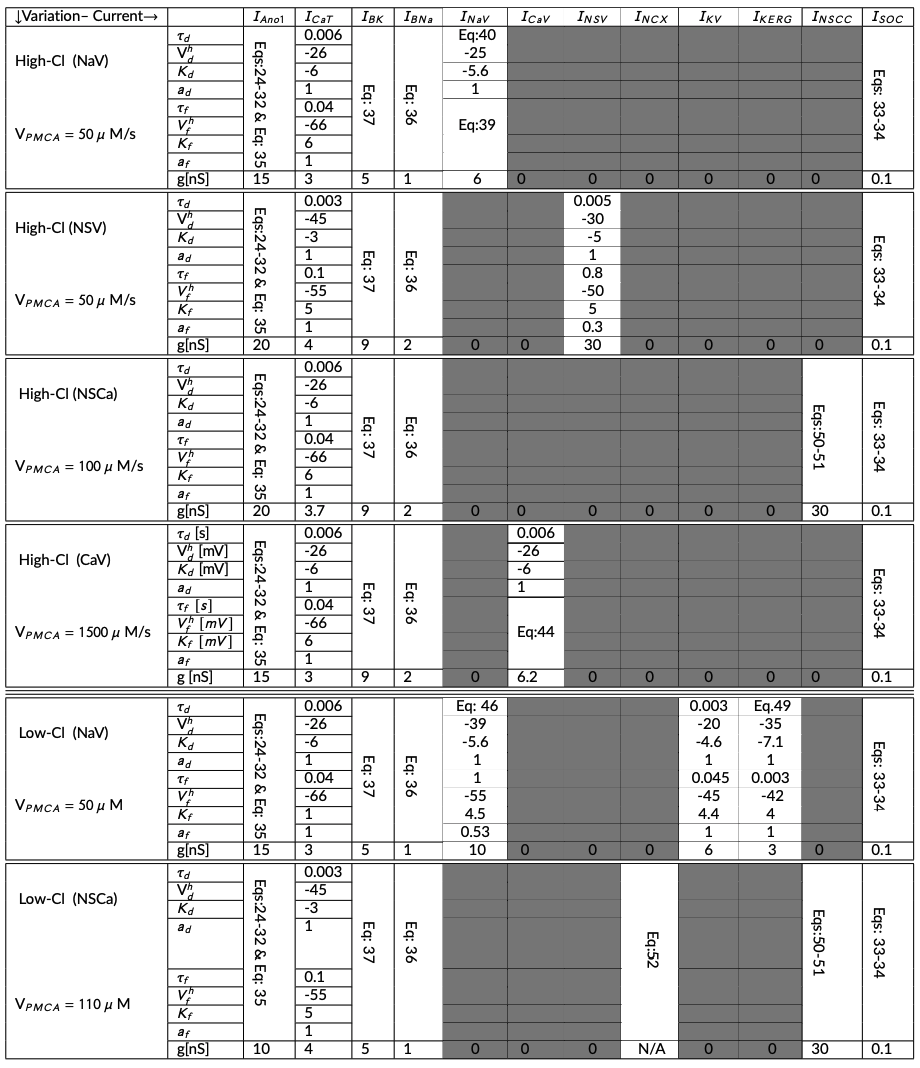
\includegraphics{table3.png}
\centering
\resizebox{\textwidth}{!}{
\begin{tabular}{|l|l|l|l|l|l|a|l|a|a|a|a|l|l|}
\hline
$\downarrow$Variation--\ Current$\rightarrow $ &  & $I_{Ano1}$ & $I_{CaT}$ & $I_{BK}$&	$I_{BNa}$ &	 \cellcolor{white}$I_{NaV}$ &	 \cellcolor{white}	$I_{CaV}$ &		 \cellcolor{white}$I_{NSV}$ &	 \cellcolor{white} $I_{NCX}$ &	 \cellcolor{white} $I_{KV}$ &	 \cellcolor{white}	$I_{KERG}$ & $I_{NSCC}$ & $I_{SOC}$  \\ \hline
% VPMCA=$50\mu$ M/s
\multirow{4}{*}{High-Cl \ (NaV)} & {$\tau_{d}$}  & \multirow{8}{*}{\begin{turn}{-90} Eqs:24-32 $\&$ Eq: 35  \end{turn}}  & 0.006 & \multirow{8}{*}{\begin{turn}{-90}  Eq: 37 \end{turn}} & \multirow{8}{*}{\begin{turn}{-90}  Eq: 36 \end{turn}} & \cellcolor{white} Eq:40 & \cellcolor{gray} &  &  &  &  & \cellcolor{gray}& \multirow{8}{*}{\begin{turn}{-90} Eqs: 33-34 \end{turn}}  \\ \cline{2-2} \cline{4-4} \cline{7-8} \cline{9-13}
 & {V$^{h}_{d}$} & & -26 & & & \cellcolor{white}-25 &\cellcolor{gray} &  & & & & \cellcolor{gray} &  \\ \cline{2-2} \cline{4-4} \cline{7-8} \cline{9-13}
 
 & $K_{d}$  &  & -6 &  &  & \cellcolor{white}-5.6  &\cellcolor{gray}  &  &  &  &  &\cellcolor{gray}  &  \\ \cline{2-2} \cline{4-4} \cline{7-8} \cline{9-13}
 & $a_{d}$  &  & 1 &  &  &  \cellcolor{white}1 & \cellcolor{gray} &  &  &  &  & \cellcolor{gray}  &  \\ \cline{2-2} \cline{4-4} \cline{7-8} \cline{9-13}
 \multirow{4}{*}{V$_{PMCA}=50 \ \mu$ M/s} & $\tau_{f}$   &  & 0.04  &  &  &  \cellcolor{white}    & \cellcolor{gray} &  &  &  &  & \cellcolor{gray} &  \\ \cline{2-2} \cline{4-4} \cline{8-8} \cline{9-13}
 & $V^{h}_{f}$  &  & -66 &  &  &\cellcolor{white}  Eq:39 &\cellcolor{gray}  &  &  &  &  & \cellcolor{gray} &  \\ \cline{2-2} \cline{4-4} \cline{8-8} \cline{9-13}
 & $K_{f}$  &  & 6 &  &  & \cellcolor{white} & \cellcolor{gray} &  &  &  &  & \cellcolor{gray} &  \\ \cline{2-2} \cline{4-4} \cline{8-8} \cline{9-13}
 & $a_{f}$  &  & 1 &  &  &\cellcolor{white}  & \cellcolor{gray} &  &  &  &  & \cellcolor{gray} &  \\  \cline{2-14}
 & g[nS]  &	15 &	3	& 5 & 1 &\cellcolor{white}	6 &	\cellcolor{gray}0 &	0 &	0 &	0 &	0 &	\cellcolor{gray}0 & 0.1   \\ \hline\hline
\multirow{4}{*}{High-Cl\ (NSV)} & {$\tau_{d}$}  & \multirow{8}{*}{\begin{turn}{-90} Eqs:24-32 $\&$ Eq: 35  \end{turn}}  & 0.003 & \multirow{8}{*}{\begin{turn}{-90}  Eq: 37 \end{turn}} & \multirow{8}{*}{\begin{turn}{-90}  Eq: 36 \end{turn}} &  & \cellcolor{gray} & \cellcolor{white}0.005  &  &  &  & \cellcolor{gray} & \multirow{8}{*}{\begin{turn}{-90} Eqs: 33-34 \end{turn}}  \\ \cline{2-2} \cline{4-4} \cline{7-8} \cline{8-13}
 & {V$^{h}_{d}$} & & -45 & & & &\cellcolor{gray} &  \cellcolor{white}-30 & & & & \cellcolor{gray}&  \\ \cline{2-2} \cline{4-4} \cline{7-8} \cline{9-13}
 
 & $K_{d}$  &  & -3 &  &  &  &\cellcolor{gray}  & \cellcolor{white} -5  &  &  &  & \cellcolor{gray}&  \\ \cline{2-2} \cline{4-4} \cline{7-8} \cline{9-13}
 & $a_{d}$  &  & 1 &  &  &  &\cellcolor{gray}  & \cellcolor{white}1  &  &  &  & \cellcolor{gray}&  \\ \cline{2-2} \cline{4-4} \cline{7-8} \cline{9-13}
 \multirow{4}{*}{V$_{PMCA}=50 \ \mu$ M/s} & $\tau_{f}$   &  & 0.1  &  &  &  &\cellcolor{gray}  & \cellcolor{white}0.8   &  &  &  &\cellcolor{gray} &  \\ \cline{2-2} \cline{4-4} \cline{7-8} \cline{9-13}
 & $V^{h}_{f}$  &  & -55 &  &  &  & \cellcolor{gray} &\cellcolor{white}-50  &  &  &  & \cellcolor{gray} &  \\ \cline{2-2} \cline{4-4} \cline{7-8} \cline{9-13}
 & $K_{f}$  &  & 5 &  &  &  &\cellcolor{gray}  & \cellcolor{white}5 &  &  &  & \cellcolor{gray} &  \\  \cline{2-2} \cline{4-4} \cline{7-8} \cline{9-13}
 & $a_{f}$  &  & 1 &  &  &  & \cellcolor{gray} &  \cellcolor{white}0.3 &  &  &  &\cellcolor{gray} &  \\ \cline{2-14}
 & g[nS]  &	20 &	4	& 9 &	2 &0 &\cellcolor{gray}		0 &	\cellcolor{white}30 &	0 &	0 &	0 &\cellcolor{gray} 0 & 0.1  \\ \hline \hline

\multirow{4}{*}{ High-Cl\ (NSCa)} & {$\tau_{d}$}  & \multirow{8}{*}{\begin{turn}{-90} Eqs:24-32 $\&$ Eq: 35  \end{turn}}  & 0.006 & \multirow{8}{*}{\begin{turn}{-90}  Eq: 37 \end{turn}} & \multirow{8}{*}{\begin{turn}{-90}  Eq: 36 \end{turn}} &  &  \cellcolor{gray}&  &  &  &  &  \multirow{8}{*}{\begin{turn}{-90} Eqs:50-51  \end{turn} }  & \multirow{8}{*}{\begin{turn}{-90} Eqs: 33-34  \end{turn}}  \\ \cline{2-2} \cline{4-4} \cline{7-12}
 & {V$^{h}_{d}$} & & -26 & & & &\cellcolor{gray} &  & & & &  &  \\ \cline{2-2} \cline{4-4} \cline{7-12}
 
 & $K_{d}$  &  & -6 &  &  &  & \cellcolor{gray} &  &  &  &  &  &  \\ \cline{2-2} \cline{4-4} \cline{7-12}
 & $a_{d}$  &  & 1 &  &  &  & \cellcolor{gray} &  &  &  &  &  &  \\ \cline{2-2} \cline{4-4} \cline{7-12}
 \multirow{4}{*}{V$_{PMCA}=100 \ \mu$ M/s} & $\tau_{f}$   &  & 0.04  &  &  &  & \cellcolor{gray} &  &  &  &  &  &  \\ \cline{2-2} \cline{4-4} \cline{7-12}
 & $V^{h}_{f}$  &  & -66 &  &  &  & \cellcolor{gray} &  &  &  &  &  &  \\ \cline{2-2} \cline{4-4} \cline{7-12} 
 & $K_{f}$  &  & 6 &  &  &  &  \cellcolor{gray}&  &  &  &  &  &  \\ \cline{2-2} \cline{4-4} \cline{7-12}
 & $a_{f}$  &  & 1 &  &  &  & \cellcolor{gray} &  &  &  &  &  &  \\ \cline{2-14}
 & g[nS]  &	20 &	3.7	& 9 &	2 &	0 &	\cellcolor{gray}0 &	0 &	0 &	0 &	0 & 30 & 0.1  \\\hline
\hline \multirow{4}{*}{ High-Cl \ (CaV)} & {$\tau_{d}$\ [s]}  & \multirow{8}{*}{\begin{turn}{-90}  Eqs:24-32 $\&$ Eq: 35  \end{turn}}  & 0.006 & \multirow{8}{*}{\begin{turn}{-90}  Eq: 37 \end{turn}} & \multirow{8}{*}{\begin{turn}{-90}  Eq: 36 \end{turn}}  & & 0.006 &  &  &  &  &  \cellcolor{gray} & \multirow{8}{*}{\begin{turn}{-90}  Eqs: 33-34 \end{turn}}  \\ \cline{2-2} \cline{4-4} \cline{7-8} \cline{8-13}
 & {V$^{h}_{d}$\ [mV]} & & -26 & & & & -26 &  & & & &\cellcolor{gray}  &  \\ \cline{2-2} \cline{4-4} \cline{7-8} \cline{9-13}
 
 & $K_{d}$\ [mV]  &  & -6 &  &  &  & -6  &  &  &  &  &\cellcolor{gray}  &  \\ \cline{2-2} \cline{4-4} \cline{7-8} \cline{9-13}
 & $a_{d}$  &  & 1 &  &  &  & 1  &  &  &  &  & \cellcolor{gray}  &  \\ \cline{2-2} \cline{4-4} \cline{7-8} \cline{8-13}
\multirow{4}{*}{V$_{PMCA}=1500 \ \mu$ M/s} & $\tau_{f}\ [s]$   &  & 0.04  &  &  & \cellcolor{gray} &\multirow{4}{*}{Eq:44}  &  &  &  &  &\cellcolor{gray}  &  \\ \cline{2-2} \cline{4-4} \cline{7-7} \cline{9-13}
 & $V^{h}_{f}\ [mV]$  &  & -66 &  &  &  & &  &  &  &  &\cellcolor{gray} &  \\ \cline{2-2} \cline{4-4} \cline{7-7} \cline{9-13}
 & $K_{f}\ [mV]$  &  & 6 &  &  &  &  &  &  &  &  &\cellcolor{gray}  &  \\ \cline{2-2} \cline{4-4} \cline{7-7} \cline{9-13}
 & $a_{f}$  &  & 1 &  &  &  &  &  &  &  &  &\cellcolor{gray}  &   \\  \cline{2-14}
 & g\ [nS]  &	15 &	3	& 9 & 2 &	0 &	6.2 &	0 &	0 &	0 &	0 &	\cellcolor{gray}0 & 0.1  \\ 
\hline\hline\hline\hline
   
 \multirow{4}{*}{ Low-Cl \ (NaV)} & {$\tau_{d}$}  & \multirow{8}{*}{\begin{turn}{-90} Eqs:24-32 $\&$ Eq: 35  \end{turn}}  & 0.006 & \multirow{8}{*}{\begin{turn}{-90}  Eq: 37 \end{turn}} & \multirow{8}{*}{\begin{turn}{-90}  Eq: 36 \end{turn}} & \cellcolor{white} Eq: 46  & \cellcolor{gray} &  &  &   \cellcolor{white}0.003&\cellcolor{white} Eq.49 &  \cellcolor{gray} & \multirow{8}{*}{\begin{turn}{-90} Eqs: 33-34  \end{turn}}  \\ \cline{2-2} \cline{4-4} \cline{7-8} \cline{9-13}
 & {V$^{h}_{d}$} & & -26 & & &\cellcolor{white}-39 & \cellcolor{gray}&  & &\cellcolor{white}-20& \cellcolor{white}-35 &  \cellcolor{gray} &  \\ \cline{2-2} \cline{4-4} \cline{7-8} \cline{9-13}
 
 & $K_{d}$  &  & -6 &  &  & \cellcolor{white}-5.6 & \cellcolor{gray} &  &  & \cellcolor{white}-4.6 & \cellcolor{white}-7.1  & \cellcolor{gray} &  \\ \cline{2-2} \cline{4-4} \cline{7-8} \cline{9-13}
 & $a_{d}$  &  & 1 &  &  &\cellcolor{white} 1 & \cellcolor{gray} &  &  & \cellcolor{white}1 & \cellcolor{white}1 &  \cellcolor{gray} &  \\ \cline{2-2} \cline{4-4} \cline{7-8} \cline{9-13}
  \multirow{4}{*}{V$_{PMCA}=50 \ \mu$ M}& $\tau_{f}$   &  & 0.04  &  &  &\cellcolor{white} 1  & \cellcolor{gray} &  &  &\cellcolor{white} 0.045 & \cellcolor{white}0.003 &  \cellcolor{gray} &  \\ \cline{2-2} \cline{4-4} \cline{7-8} \cline{9-13}
 & $V^{h}_{f}$  &  & -66 &  &  & \cellcolor{white}-55 & \cellcolor{gray} &  &  & \cellcolor{white}-45 &\cellcolor{white} -42 &  \cellcolor{gray} &  \\ \cline{2-2} \cline{4-4} \cline{7-8} \cline{9-13}
 & $K_{f}$  &  & 1 &  &  & \cellcolor{white}4.5 &\cellcolor{gray}  &  &  & \cellcolor{white}4.4 & \cellcolor{white}4 &  \cellcolor{gray} & \\ \cline{2-2} \cline{4-4} \cline{7-8} \cline{9-13}
 & $a_{f}$  &  & 1 &  &  & \cellcolor{white}0.53 & \cellcolor{gray} &  &  & \cellcolor{white}1 & \cellcolor{white}1 & \cellcolor{gray} &  \\ \cline{2-14}
 & g[nS]  &	15 &	3	& 5 &	1 &\cellcolor{white}	10 &\cellcolor{gray}	0 &	0 & 0 &	\cellcolor{white}6 &\cellcolor{white}	3 & \cellcolor{gray} 	0 & 0.1  \\ \hline\hline
 
 \multirow{4}{*}{ Low-Cl \ (NSCa)} & {$\tau_{d}$}  & \multirow{8}{*}{\begin{turn}{-90} Eqs:24-32 $\&$ Eq: 35  \end{turn}}  & 0.003 & \multirow{8}{*}{\begin{turn}{-90}  Eq: 37 \end{turn}} & \multirow{8}{*}{\begin{turn}{-90}  Eq: 36 \end{turn}} & & \cellcolor{gray}   &  &\cellcolor{white}&  &  & \multirow{8}{*}{\begin{turn}{-90} Eqs:50-51  \end{turn} } & \multirow{8}{*}{\begin{turn}{-90} Eqs: 33-34 \end{turn}}  \\ \cline{2-2} \cline{4-4} \cline{7-9} \cline{11-12}
 & {V$^{h}_{d}$} & & -45 & & & & \cellcolor{gray}  &  & \cellcolor{white}& & &  &  \\ \cline{2-2} \cline{4-4} \cline{7-9} \cline{11-12}
 
 & $K_{d}$  &  & -3 &  &  &  &  \cellcolor{gray}  &  &\cellcolor{white}  &  &  & &  \\ \cline{2-2} \cline{4-4} \cline{7-9} \cline{11-12}
 & $a_{d}$  &  & 1 &  &  &  & \cellcolor{gray}   &  & \cellcolor{white} \begin{turn}{-90} Eq:52  \end{turn}  &  &  & &  \\ \cline{2-2} \cline{4-4} \cline{7-9} \cline{11-12}
 \multirow{4}{*}{V$_{PMCA}=110 \ \mu$ M} & $\tau_{f}$   &  & 0.1  &  &  &  &  \cellcolor{gray}  &  &  \cellcolor{white} &  &  & &  \\ \cline{2-2} \cline{4-4} \cline{7-9} \cline{11-12}
 & $V^{h}_{f}$  &  & -55 &  &  &  &  \cellcolor{gray}  &  & \cellcolor{white} &  &  & &  \\ \cline{2-2} \cline{4-4} \cline{7-9} \cline{11-12}
 & $K_{f}$  &  & 5 &  &  &  &  \cellcolor{gray}  &  & \cellcolor{white} &  &  &  &  \\ \cline{2-2} \cline{4-4} \cline{7-9} \cline{11-12}
 & $a_{f}$  &  & 1 &  &  &  & \cellcolor{gray}   &  &  \cellcolor{white} &  &  & &  \\ \cline{2-14}
 & g[nS]  &	10 &	4	& 5 &	1 &	0 &	 \cellcolor{gray} 0 & 0 & \cellcolor{white} N/A &	0 &	 \cellcolor{gray} 0 & 30 & 0.1  \\ \hline

\end{tabular}}
\end{table}
% \end{landscape}
\subsection{Model Results}
We employed the Engauge Digitizer software \citep{mark_mitchell_2020_3941227} to extract the data from all figures from  \citet{lees2014computational} to present alongside the results of the present work. The reproduction of all figures of \citet{lees2014computational} is given in Figures 1-3, which show good agreement against the data of the primary paper. Solid lines show the output from this curation effort, and stars show discrete points found by the Engauge Digitizer of the figures in the primary paper.
\begin{figure}[ht!]\centering
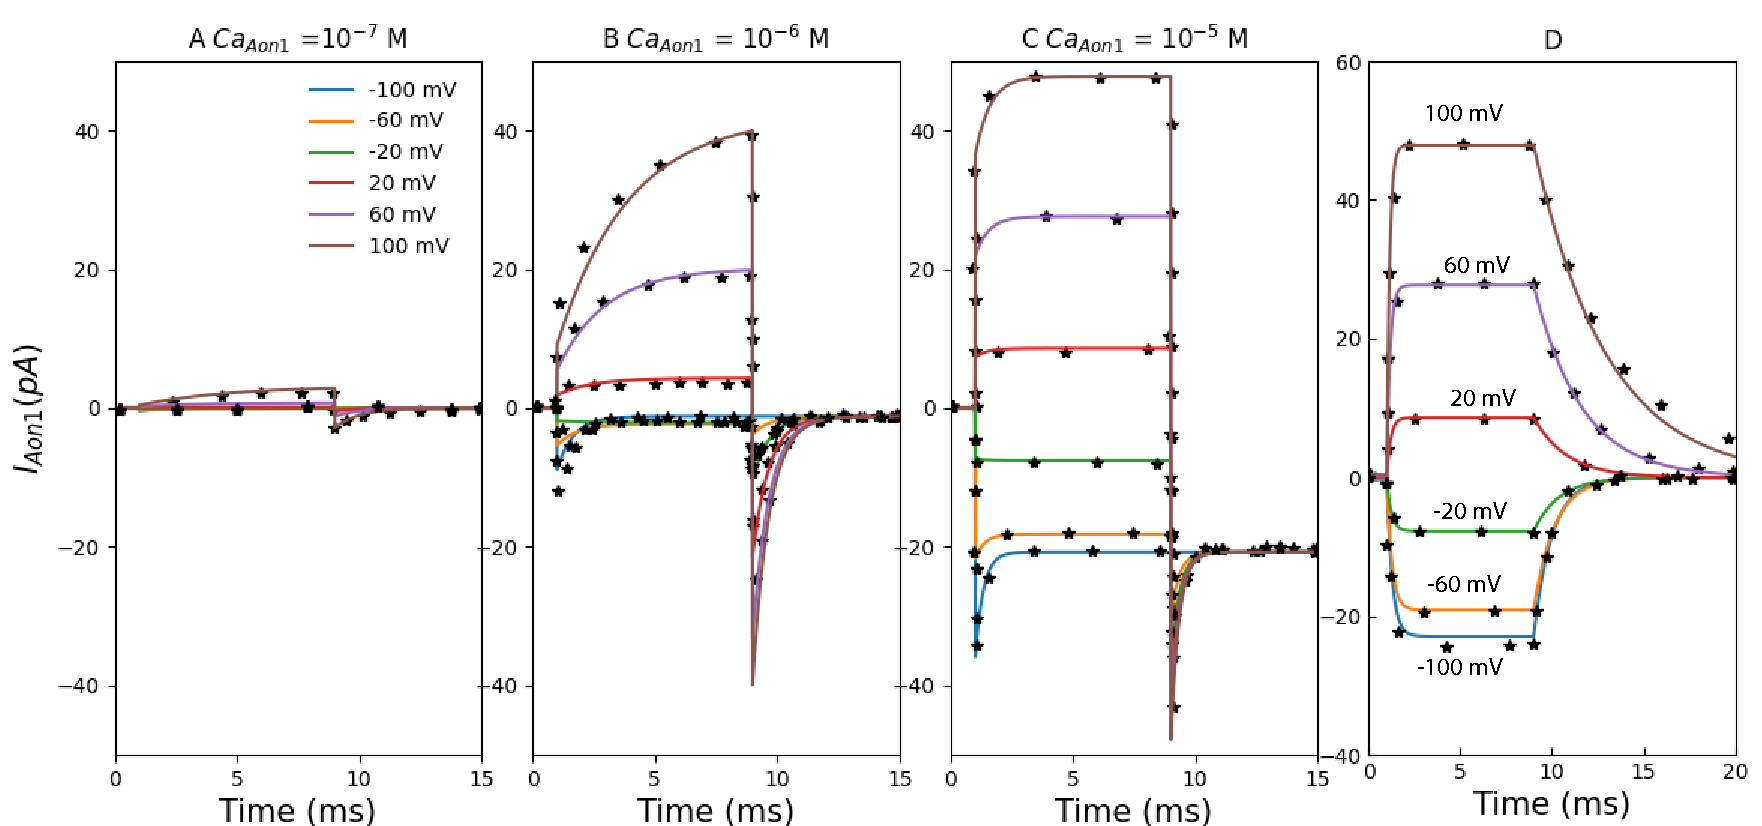
\includegraphics[width=1.00\linewidth]{Figure3.pdf}
\caption{The primary data (*) of \cite[Figure 3]{lees2014computational} with our reproduction of all subfigures. To reproduce \citet[Figure 3]{lees2014computational}, use the Python script \texttt{IAno1.py} to produce the simulation results and \texttt{Plot\_Fig3\_Ano1.py} to plot the results. A–C: simulated voltage-clamp experiments to test the response of the Ano1 model to the voltage protocol.}
\label{fig:fig3}
\end{figure}
\newpage
\begin{figure}[ht!]%\centering
\hspace*{-2.6cm} 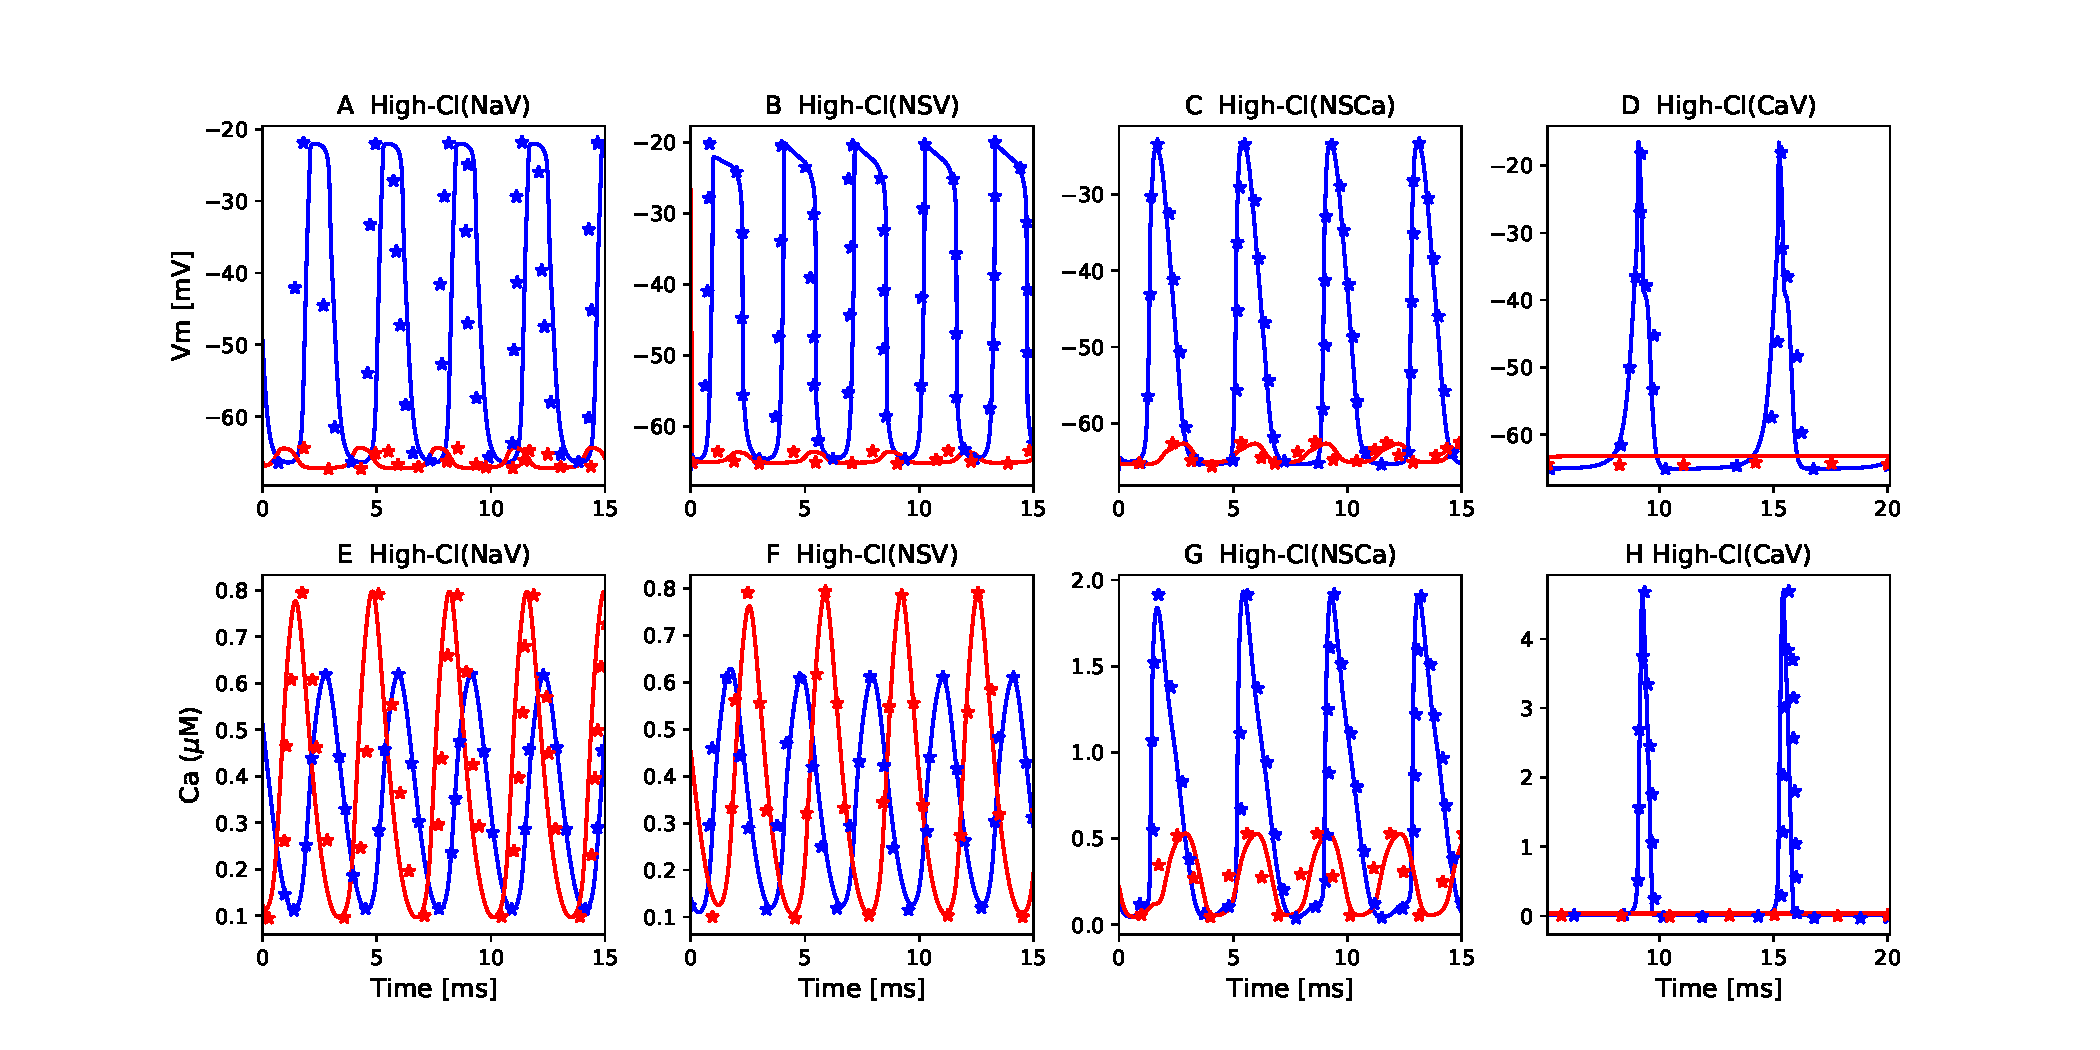
\includegraphics[scale=0.55]{Figure4.pdf}
\caption{The primary data (*) of \cite[Figure 4]{lees2014computational} with our reproduction of all subfigures. To reproduce \cite[Figure 4]{lees2014computational}, use the Python script \texttt{ICC\_Lees\_Green.py} to produce the simulation results and \texttt{Plot\_Fig4\_ICC.py} to plot the results. A-H: membrane potentials were simulated using the wild-type (WT) and Ano1 knockout (KO) scenarios (blue and red lines, respectively).}
\label{fig:fig4}
\end{figure}

\begin{figure}[ht!]%\centering
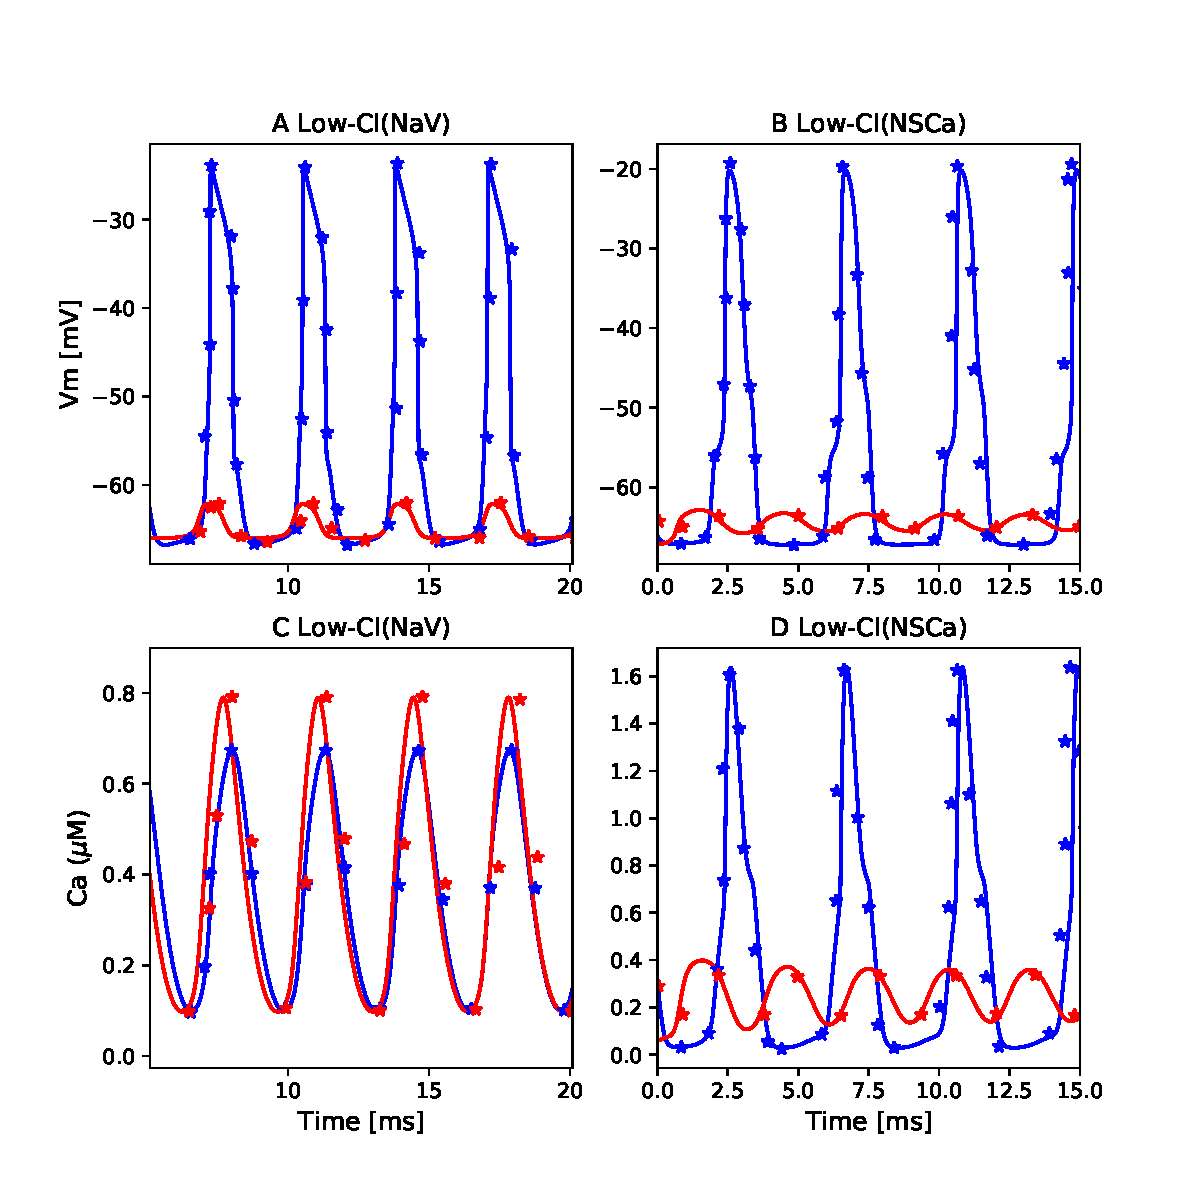
\includegraphics[width=1\linewidth]{Figure5.pdf}
\caption{The primary data (*) of  \cite[Figure 5]{lees2014computational} with our reproduction of all subfigures. To reproduce \cite[Figure 5]{lees2014computational}, use the Python script \texttt{ICC\_Lees\_Green.py} to produce the simulation results and \texttt{Plot\_Fig5\_ICC.py} to plot the results. A-D: membrane potentials simulated using the wild-type (WT) and Ano1 knockout (KO) scenarios (blue and red lines, respectively).}
\label{fig:fig5}
\end{figure}



\section{Discussion}
We demonstrated that most results of \citet{lees2014computational} can be reproduced given some added equations (\autoref{eq:0}) and adjustments (\autoref{tab:Inconsistency}) made to model parameter values. We implemented the model \citep{lees2014computational} using CellML, replicated all the model behaviors reported in the primary paper, and summarized detailed
experiment settings for simulation in \autoref{Computational-Simulation}. While we are generally able to reproduce the simulation results there are some cases where the results presented here are not identical. The reason for this is the lack of information about the initial conditions from the primary paper leading to slight phase shifts in the oscillatory behaviour as the simulations are not starting from the same initial state. These differences do not impact their interpretation and the conclusions drawn in the primary paper of \citet{lees2014computational}.
Python code was needed in some cases and can be found at \url{https://models.physiomeproject.org/workspace/762}. 
As this paper follows the tenets of FAIR \citep{wilkinson2016fair}, further credibility is lent to the primary models.


\section{Acknowledgements}
The authors gratefully acknowledge the support of the Ministry of Business, Innovation and Employment’s
Catalyst Strategic Fund (12 Labours).

\FloatBarrier



\bibliography{ref}

\end{document}